\documentclass[12pt]{article}

\usepackage[utf8]{inputenc}

\title{Rapid shortening at the eastern margin of the Tibetan plateau prior to the 2008 Mw=7.9 Wenchuan earthquake}
\author{T. Ben Thompson, Brendan J. Meade}
\date{September 2014}
\usepackage{graphicx}
\usepackage[margin=1.0in]{geometry}
\usepackage[nomarkers,figuresonly]{endfloat}
\usepackage{setspace}
\usepackage{natbib}
\doublespacing

\begin{document}

\maketitle

\section{Abstract}
The Longmen Shan is the steepest topographic front of the India-Asia collision and was the site of the Mw=7.9 Wenchuan earthquake. Shortening estimates across the Longmen Shan provide strain accumulation rates and clarify the eastward extrusion of the Tibetan plateau. Here, to explain the interseismic GPS velocities across the greater Longmen Shan region, we develop a boundary element model including earthquake cycle effects, topography, the westward dipping Beichuan fault, and a ~20 km deep, shallowly dipping, detachment. The detachment is inferred from observations of slip during and after the Wenchuan earthquake and from structural considerations. Previous analyses which neglected the detachment and earthquake cycle effects have found shortening rates near zero. In contrast, we find that interseismic GPS data are consistent with a shortening rate of 6$\pm$2 mm/yr. These results suggest that the Longmen Shan is an active fold-and-thrust belt with Wenchuan style earthquake recurrence intervals of $<$600 years.

\section{Introduction}
The Longmen Shan range is located on the eastern margin of the Tibetan and rises 4000m over 30km.  The 2008 $\mathrm{M_w}$ 7.9 Wenchuan earthquake ruptured 250km along strike on the Beichuan and Pengguan faults, resulting in approximately 70000 fatalities. Prior geodetic estimates suggest almost zero horizontal shortening \citep{king97, chen00, shen05, Meade07c, Loveless2011}, in contrast with the dominant thrust slip-sense during the Wenchuan rupture.  Other authors reconcile the lack of shortening with the steep topography by appealing a lower crustal inflation tectonic model for the eastern Tibetan Plateau \citep{royden97, bird91, Burchfiel2008a}.  However, the magnitude and location of the Wenchuan earthquake suggest a more typical fold-and-thrust belt.  Using seismic reflection data, \citet{hubbard09} find a well-developed fold-and-thrust fault system geometry with long-term shortenings up to 100\%.  A growing body of literature supports this interpretation. \citet{Fielding2012a} interpret satellite gravity-field data to infer that mass of the Longmen Shan is supported by a flexed Sichuan Basin.  This fold-and-thrust structure may extend deep into the plateau as suggested by seismic tomography, reflection, magnetotelluric data and studies of the Longriba fault zone 200km northwest of the Longmen Shan \citep{Xu2008, Zhang2009, Zhao2012, Ren2013, Guo2013}. (LOTS TO EXTEND HERE, SPACE?)

However, it remains to be explained how slow present-day geodetic shortening estimates can be reconciled with the Wenchuan earthquake and the large structurally-observed shortening. Prior estimates can be categorized into those that neglect earthquake cycle effects, analyzing the fault slip-deficit without no explicit model of the geometry or tectonics, \citep{chen00, shen05} and those that use block models, which normally assume a simplified fault geometry \citep{Meade07c, Loveless2011, Burchfiel2008a}. \citet{Loveless2011} report the highest shortening rate of 3.2 mm/yr.  Here, we present a model that includes earthquake cycle effects to explain the regional geodetic velocities as the result of a complex interseismically locked fault geometry, including a 20km deep detachment and the range-front thrust Beichuan fault.  This geometry is consistent with the inference of 2-6m of slip of a 20km deep detachment that extends 90km northwest using InSAR measurements and post-Wenchuan GPS observations \citep{Qi2011}. \citet{Fielding2013b} also include a detachment fault plane in their joint geodetic-teleseismic coseismic slip inversion. Further, this geometry is consistent with structural interpretations \citep{Hubbard2010, Li2010}. Using this range-front thrust plus detachment geometry, we infer an average horizontal shortening between the TIbetan Plateau using interseismic GPS data collected prior to the Wenchuan earthquake.  Next, we show how this geometry can drive the steep velocity gradients far to the northwest of the range front, thus explaining the absence of a range-front interseismic velocity gradient. Importantly, this model provides increased estimates of seismic hazard. This model proposes that strain accumulates up to 300km from the margin of the Tibetan plateau while being released at the Longmen Shan range front, thus providing a unified theory of the Longmen Shan earthquake cycle. 

\section{Geodetic analysis of Longmen Shan shortening}

\begin{figure}[h!]
    \centering
    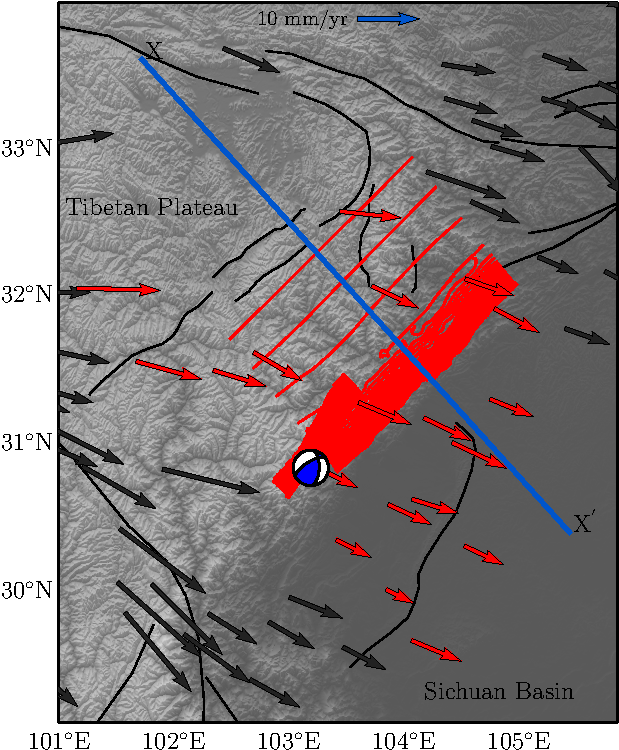
\includegraphics{figs/lms_map_all.pdf}
    \caption{A map of the Longmen Shan region with the basemap showing shaded relief. The focal mechanism plot is located at the epicenter of the Wenchuan earthquake, while the thicker red line shows the surface trace of rupture. The thin red lines show 1km depth contours of our model geometry. GPS velocity vectors are colored black if they are not included in our parameter estimation and red if they are included. The blue line shows the two-dimensional cross-section we study. Thin black lines indicate other significant faults in the region.}
    \label{fig:regional_map}
\end{figure}

The fault geometry we consider is derived from a Community Fault Model for the Longmen Shan and Sichuan Basin region being actively developed (Plesch and Shaw, personal communication).  This geometry is derived from structural interpretation of both seismic reflection surverys and surface geology \citep{Hubbard2010}.  We make no modifications to this geometry except to take a fault-perpindicular cross-section. The depth and dip of the detachment are similar to the best-fitting surface found by \citet{Qi2011}. The cross-section and geometry with depth contours are shown in Figure \ref{fig:regional_map}.

Because this model includes a deep detachment, we must include interseismic GPS data deep into the interior of the Tibetan Plateau. We study GPS observations collected prior to the Wenchuan earthquake \citep{apel06,Banerjee2008,calais06, gan07, vigny03}, assembled into a single reference frame by \citet{Loveless2011}. These velocities are shown in Figure \ref{fig:regional_map} along with the site of the Wenchuan earthquake and other regional faults \citep{Taylor09}. We include in the estimation velocities that are within the potential far-field influence of a deep detachment under the easternmost Tibetan Plateau. We exclude velocities that are near major faults like the Xianshuihe fault or the Kunlun fault. Later, we demonstrate that our results are reasonably robust to the specific data set that is studied. Addition of more recent observations could bias our results due to possible postseismic transient deformation.

To analyze these data, we use new quasistatic elastic boundary element software. An important feature of our tool is the inclusion of accurate surface topography in steep mountain ranges or Earth curvature in large-scale problems. In addition, we can accurately reproduce half-space solutions to very high precision. The steep topography of the Longmen Shan range front is included via the SRTM30\_PLUS digital elevation dataset \citep{Becker2009}.

\begin{figure}[h!]
    \centering
    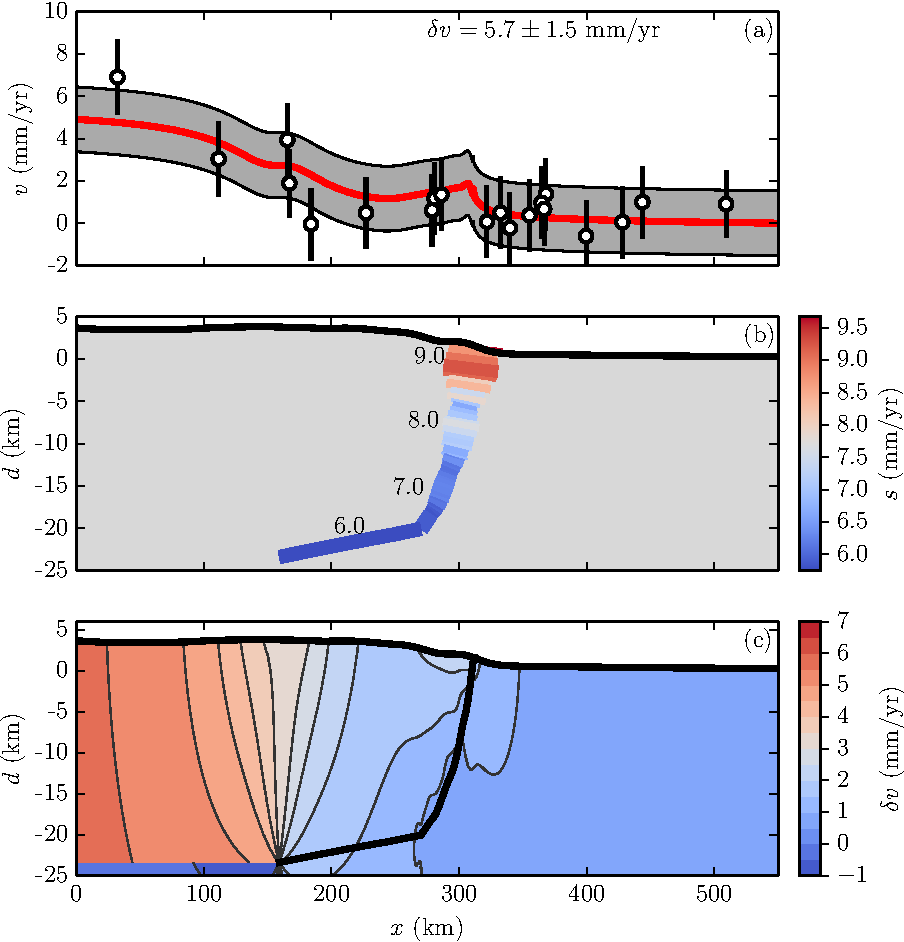
\includegraphics{figs/stack_figure_all_details.pdf}
    \caption{a) Observed profile-parallel horizontal observed velocities are shown in black with 68\% confidence errorbars. Model-predicted velocities are shown by the red line with the surrounding gray region showing a 68\% confidence interval. b) Model geometry with colors and width along the locked fault showing predicted slip-deficit rates. Because shortening is the horizontal component of slip-deficit, increasing dips near the surface lead to larger slip-deficits. c) Predicted horizontal velocity as a function of depth. Note the steep velocity gradient and corresponding strain accumulation above the end of the detachment surface.}
    \label{fig:big_stack}
\end{figure}


The debate over shortening in the Longmen Shan has centered around the clear lack of velocity gradient at the range front. However, this discussion has neglected the interplay between earthquake cycle effects and fault geometry. A Beichuan-only fault geometry would predict very little deformation beyond 100km \citep{savage83}, leading to the exclusion of velocities beyond this range. Both the observed and predicted profile-parallel velocities shown in Figure \ref{fig:big_stack}a make clear that such an estimate would result in a near-zero shortening estimate.

A locked detachment, however, drives the predicted location of steep velocity gradient far to the northwest as shown by Figure \ref{fig:big_stack}a. The best-fit shortening rate for the Longmen Shan region is 5.7 $\pm$ 1.5 mm/yr. For discussion of seismic hazard, shortening must be translated to fault-parallel slip-deficit. Figure \ref{fig:big_stack}b shows the increase in slip-deficit from ~6.0 mm/yr up to 9.5 mm/yr at the surface. Figure \ref{fig:big_stack}c shows the horizontal velocities as a function of depth, demonstrating that the velocity gradients derive from the detachment tip. The smoothing behavior of an elastic Earth prevents distinguishing between a sharp drop in slip-deficit or a gradual change over many kilometers. These results demonstrate the mechanism by which it is possible for interseismic strain accumulation to occur far from the range-front structures on which it is released.

The primary uncertainty in our shortening estimate is the lack of good constraints on the detachment geometry in the hinterland. However, assuming the geometry is correct, two further forms of error are evident. First, the uncertainty in true interseismic velocities is propagated through to the estimated shortening, resulting in the gray region of uncertainty in Figure \ref{fig:big_stack}a. Further, the sparsity of observations suggests that certain observations may undue influence on the shortening estimate. Excluding the northwest-most observation decreases the best-fit shortening to 3.9 $\pm$ 1.9 mm/yr. The least squares uncertainty is increased (from 1.5 mm/yr to 1.9 mm/yr) because the northwestern portion of velocities are poorly constrained once the observation is excluded. 

Figure \ref{fig:distribution} shows a more complete analysis of the effect of case resampling the observations on the slip-deficit rate. Because there only $2^{20} = 1.048 $ million different possible subsets of the observations, we perform a complete case resampling bootstrap. Subsequently, we sample jointly from this distribution and the distribution of surface-area weighted fault depths. This analysis demonstrates that the majority of the slip-deficit-depth probability landscape lies at slip-deficit rate between 4 and 6 mm/yr while certain parts of the geometry (the range-front) have much faster slip-deficit rates.

\begin{figure}[h!]
    \centering
    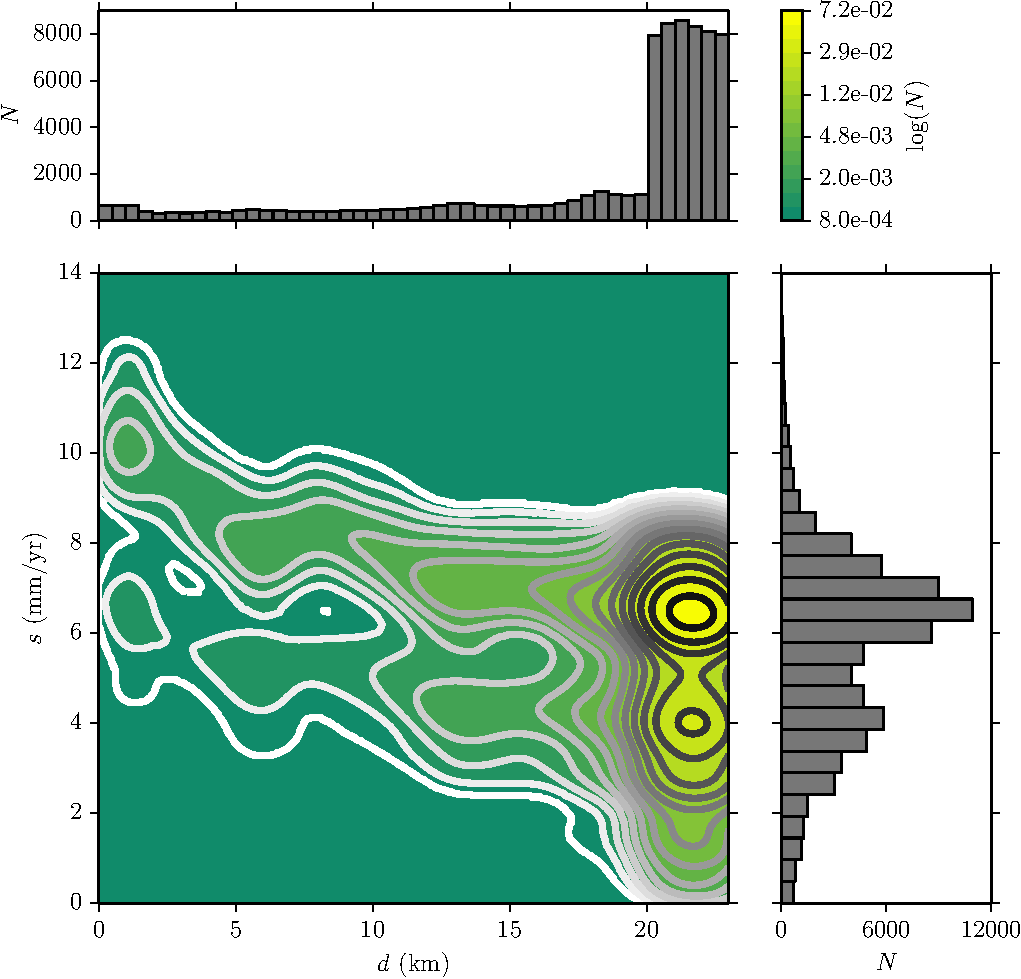
\includegraphics{figs/depth_slip_contour.pdf}
    \caption{The depth-slip-deficit probability landscape. The upper histogram is the projection of the contour plot onto a depth histogram, demonstrating that the majority of the fault surface area lies on the deep detachment. The right histogram is the projection of the contour plot onto a slip-rate histogram showing that the majority of fault surface area is slipping at rates near 6 mm/yr.}
    \label{fig:distribution}
\end{figure}

\section{Implications for the Longmen Shan earthquake cycle}
The striking feature of Figure \ref{fig:big_stack}a is the lack of a range-front geodetic signature of shortening. 

Model without topography do not have a local minimum northwest of the Beichuan, indicating the relevance of topography in crustal deformation.

This far-field deformation is consistent with vertical leveling data that suggests a vertical velocity profile that increases from the Longmen Shan range front until peaking 50km southeast of the Longriba fault zone \citep{Hao2014}. The Longriba fault zone has the wrong slip-sense (up to the south-east, \citep{Ren2013}) to accomodate such vertical deformation. No other structure is nearby. 

Figure \ref{fig:hazard} shows a summary of recurrence intervals as a function of total event slip. Our shortening estimate suggests a recurrence interval for Wenchuan-like ruptures of approximately 600 years. Recurrence for smaller events is much more frequent. This contrasts with the average recurrence of ~2000 years determined by \citep{Ran2010} for the Beichuan fault. Our estimate would predict $M_w = $9.0 ruptures on that recurrence, seemingly unlikely given the total slip and fault length required. However, our estimate is an system-wide recurrence while that paleoseismic estimate is limited by only studying one of multiple imbricated thrusts. 

There are reasons to believe that the seismic hazard estimate presented here is a low estimate.  First, coseismic and long term slip estimates include (CITE VARIOUS COSEISMIC + DENSMORE) a significant component of strike-slip motion. But, we only model horizontal shortening.  Second, our two-dimensional model assumes plane strain conditions.  The approximation will result in under-estimates of the shortening required to produce far-field velocities.  This is because the assumption is equivalent to assuming the fault geometry extends infinitely far along strike, resulting in a fault surface much larger than in reality. Third, the modeled thrust is the steeply dipping Beichuan fault. The foreland Range Front thrust or the shallow detachment beneath Chengdu dip more shallowly \citep{Hubbard2010}, producing a greater total moment deficit.  Finally, the shortening rate estimate may be low due to being estimated late in the earthquake cycle \citep{savage00}.  It is also important that the recurrence interval calculation assumed that the entire range-front was ruptured by the Wenchuan earthquake whereas the southern portion of the Longmen Shan did not rupture during the earthquake and is thought to similarly active to the portions that did rupture \citep{Li2010}. 

Approximately 150 kilometers west of the Beichuan fault, there are 3 GPS stations with similar profile location. But, the velocities are significantly different. This indicates some lateral heterogeneity not represented by our two-dimensional modelling. 



\begin{figure}[h!]
    \centering
    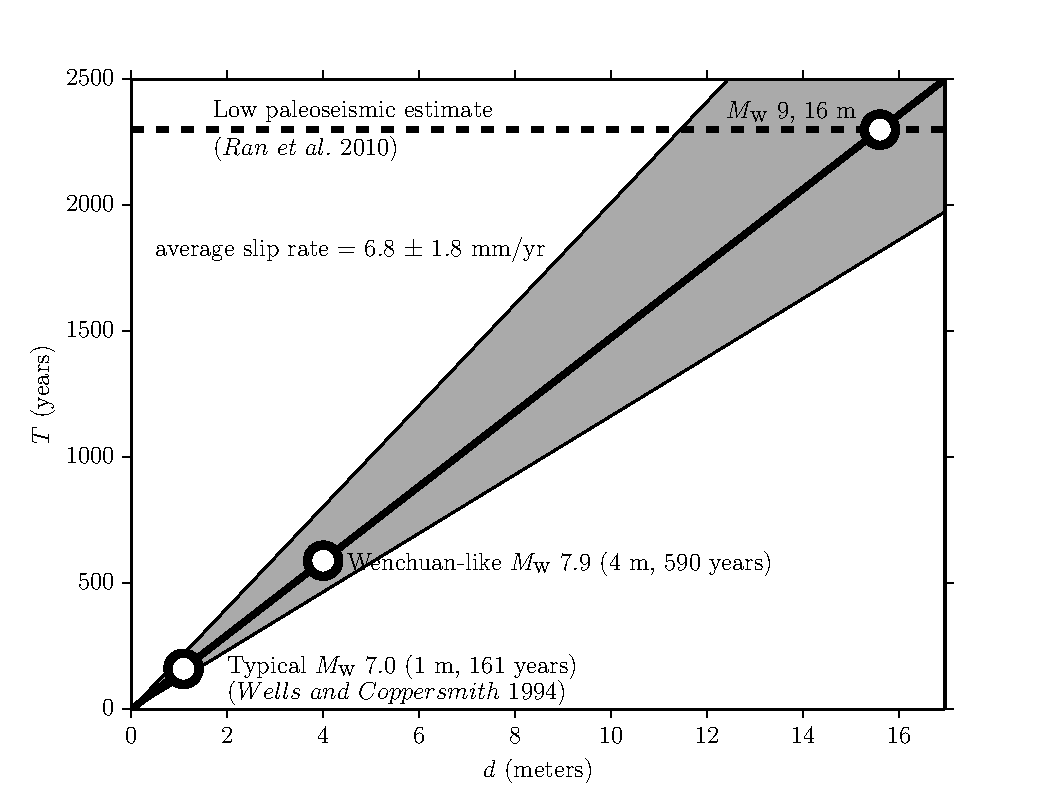
\includegraphics{figs/hazard_all_details.pdf}
    \caption{Recurrence as a function of slip, assuming the best-fit slip rate for the Beichuan fault. The gray region indicates the uncertainty implied by the error in our shortening estimate. The discrepancy between the Wenchuan-like recurrence and the paleoseismic estimate may be due to the presence of multiple active faults in the range-front.}
    \label{fig:hazard}
\end{figure}

Previous near-zero shortening estimates in the Longmen Shan are at odds with the large-moment of the Wenchuan earthquake, very steep topography, structural interpretations indicate fold-and-thrust geometry, fast erosion rates. We clarify this conflict by including earthquake cycle effects and a 20km deep detachment. Our revised interseismic shortening rate is 5.7 $\pm$ 1.5 mm/yr. This interpretation unifies models of coseismic (Wenchuan), postseismic and interseismic  based on geodetic data. Our model suggest that Wenchuan-like events have much shorter recurrence intervals.

\bibliographystyle{plainnat}
\bibliography{biblio,library}
\end{document}
